
\section{Memory Controller Design}
\label{sec:memcontrol}
\Matt{BLUE: I would not mind removing this text. RED: I will likely remove this text}
In this section, we discuss the architecture of the memory controller for the proposed memory system. This memory controller is designed to make use of the coding schemes discussed in the previous section. The architecture of the memory controller is focused on exploiting the redundant storage in the coding schemes to serve memory requests faster than an uncoded scheme. This section presents the key architectural requirements of the memory controller and potential implementations of these requirements.
%The memory design involves two key components: 1) storage space comprising of memory banks and 2) memory controller 
%The coding schemes discussed in previous section is implemented using systemC. 
%This section describes the architectural detail of how the schemes are 
%implemented using optimized algorithms. \\
%In this section, we explore the technique of dynamic coding in order to reduce 
%the memory and access overhead
%associated with the parity banks. We first discuss the scheme of dynamic coding 
%and follow it by discussing the potential benefits of prefetching the codes.\\

\subsection{Memory Controller Stages}
A general memory controller consists of three stages of processing illustrated in Figure~\ref{fig:pseudo-code}. The first stage, the {\em core arbiter}, receives memory access request from the master cores. The core arbiter then routes the requests to the proper {\em bank queue}. The bank queues are the second stage of processing, and they are responsible for storing and tracking memory requests. A memory request seeking memory located in bank $N$ will be sent to the $N$th bank queue. The {\em access scheduler} is the final stage of processing. It is responsible for scheduling the requests in the bank queues. Each memory cycle, the access scheduler generates an access pattern based on the requests present in the bank queues. The access pattern is a description of the reads or writes the memory controller will perform on the memory banks. Next, we discuss all of these three units and their functions in a greater detail.
%first level is {\em Core Arbiter }, the unit responsible for handling requests 
%from cores.  The second level is {\em Bank Arbiter} responsible for arbitrating 
%requests to banks.  The third level is {\em Access Scheduler} which schedules 
%most efficient access for each cycle.\\
%%-----------------------
\begin{figure}[htbp]
\centering
	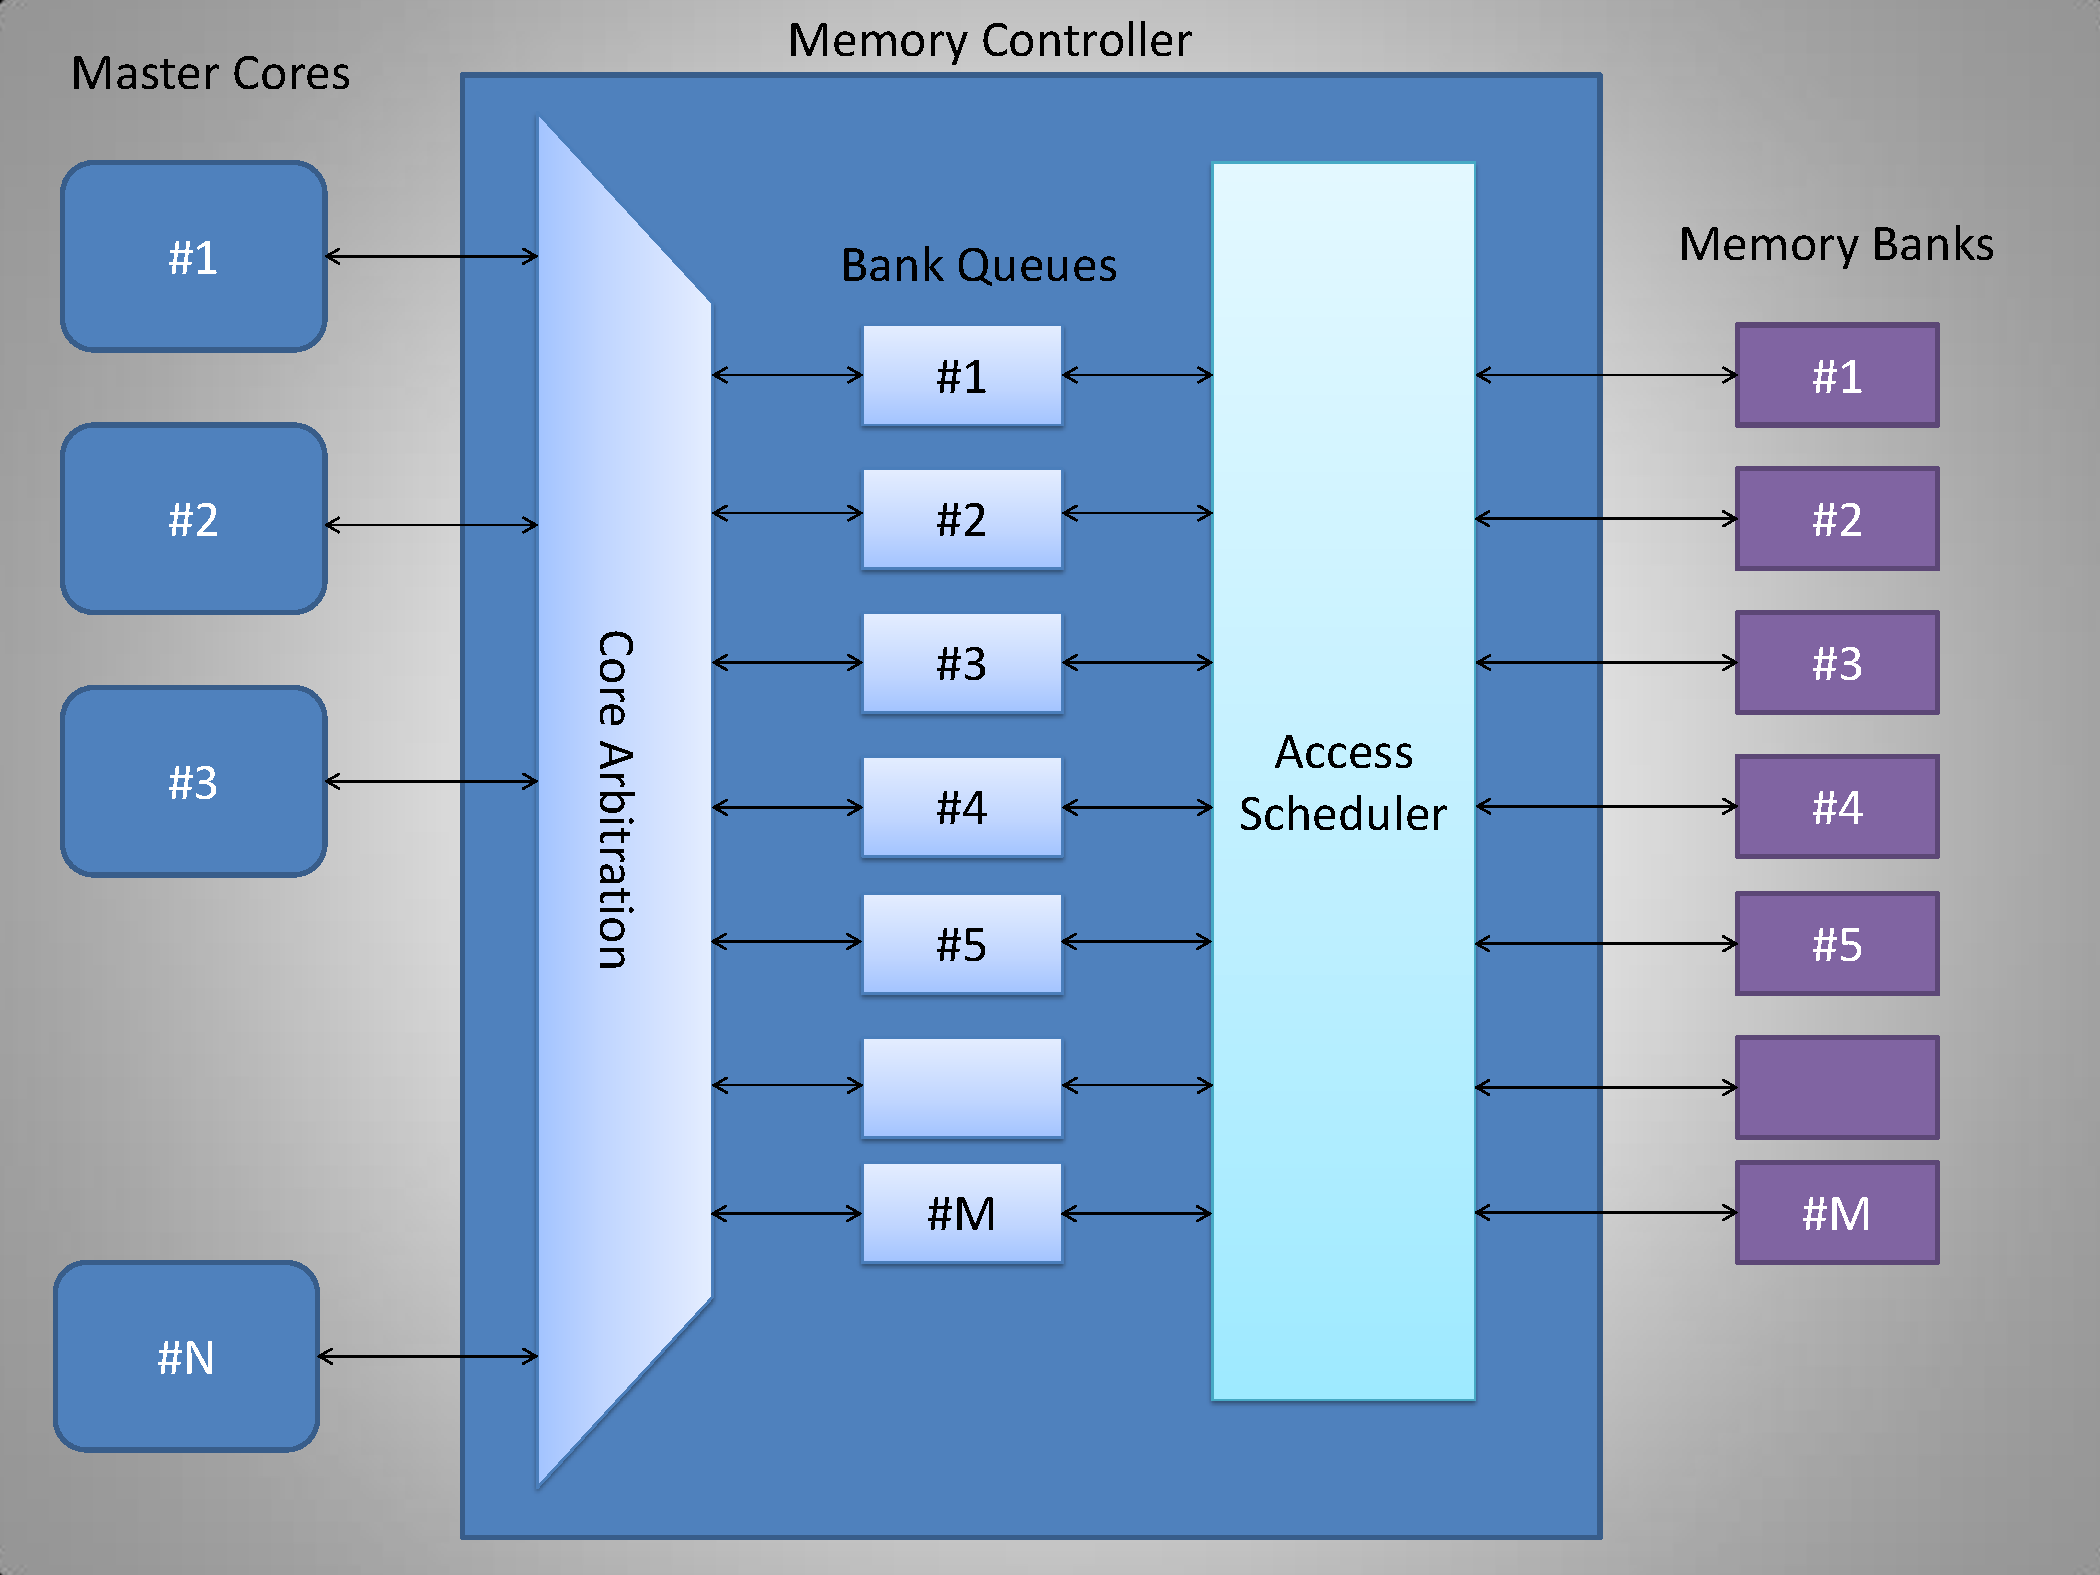
\includegraphics[width=0.7\linewidth]{fig/controllerArchitecture.pdf}
\caption{
{Architecture of Memory Controller} }
\label{fig:pseudo-code}
\end{figure}
%-------------------------
\begin{itemize}
\item \textbf{Core arbiter:~}Every clock cycle, the core arbiter receives up to one request from each core which it stores in an internal queue. The core arbiter attempts to push these request to the appropriate bank queue. If in attempting to push a request the core arbiter detects that the destination bank queue is full, the controller signals that the core is busy which stalls the core. The core arbiter is also responsible for arbitration among the access requests. It arranges the requests stored in its internal queue using a two-step priority order mechanism. It arranges the request in order of QoS priority, and it arranges requests with the same QoS priority using round-robin scheduling.

\item \textbf{Bank queues:~}Each data bank has a corresponding read queue and write queue.  The core arbiter sends memory requests to the bank queues until the queues are full. In our simulations, we use a bank queue depth of 10. 

In addition to the read and write queues, there is a single queue which holds special requests such as memory refresh requests.

\item \textbf{Access scheduler:~}The access scheduler is responsible for handling interactions with the memory banks. Every memory cycle, the access scheduler chooses to serve read requests or write requests and algorithmically determines which requests in the bank queues it will schedule. The scheduling algorithms the access scheduler uses are called pattern builders. Every memory cycle, the access scheduler invokes either the read pattern builder or the write pattern builder to schedule read or write requests respectively. A key design trade-off of the pattern builder algorithms is the relationship between the complexity of the algorithm and the number of requests the algorithm schedules.
\end{itemize}

We note that the core arbiter and bank queues should not differ much from those in a traditional setup with an uncoded storage space. The access scheduler directly interacts with the memory banks including the parity banks, so it must be designed with the proposed coding schemes in mind. The rest of this section is devoted to discussing the access scheduler in detail.


%-----------------------
\begin{figure}[tbp]
\centering
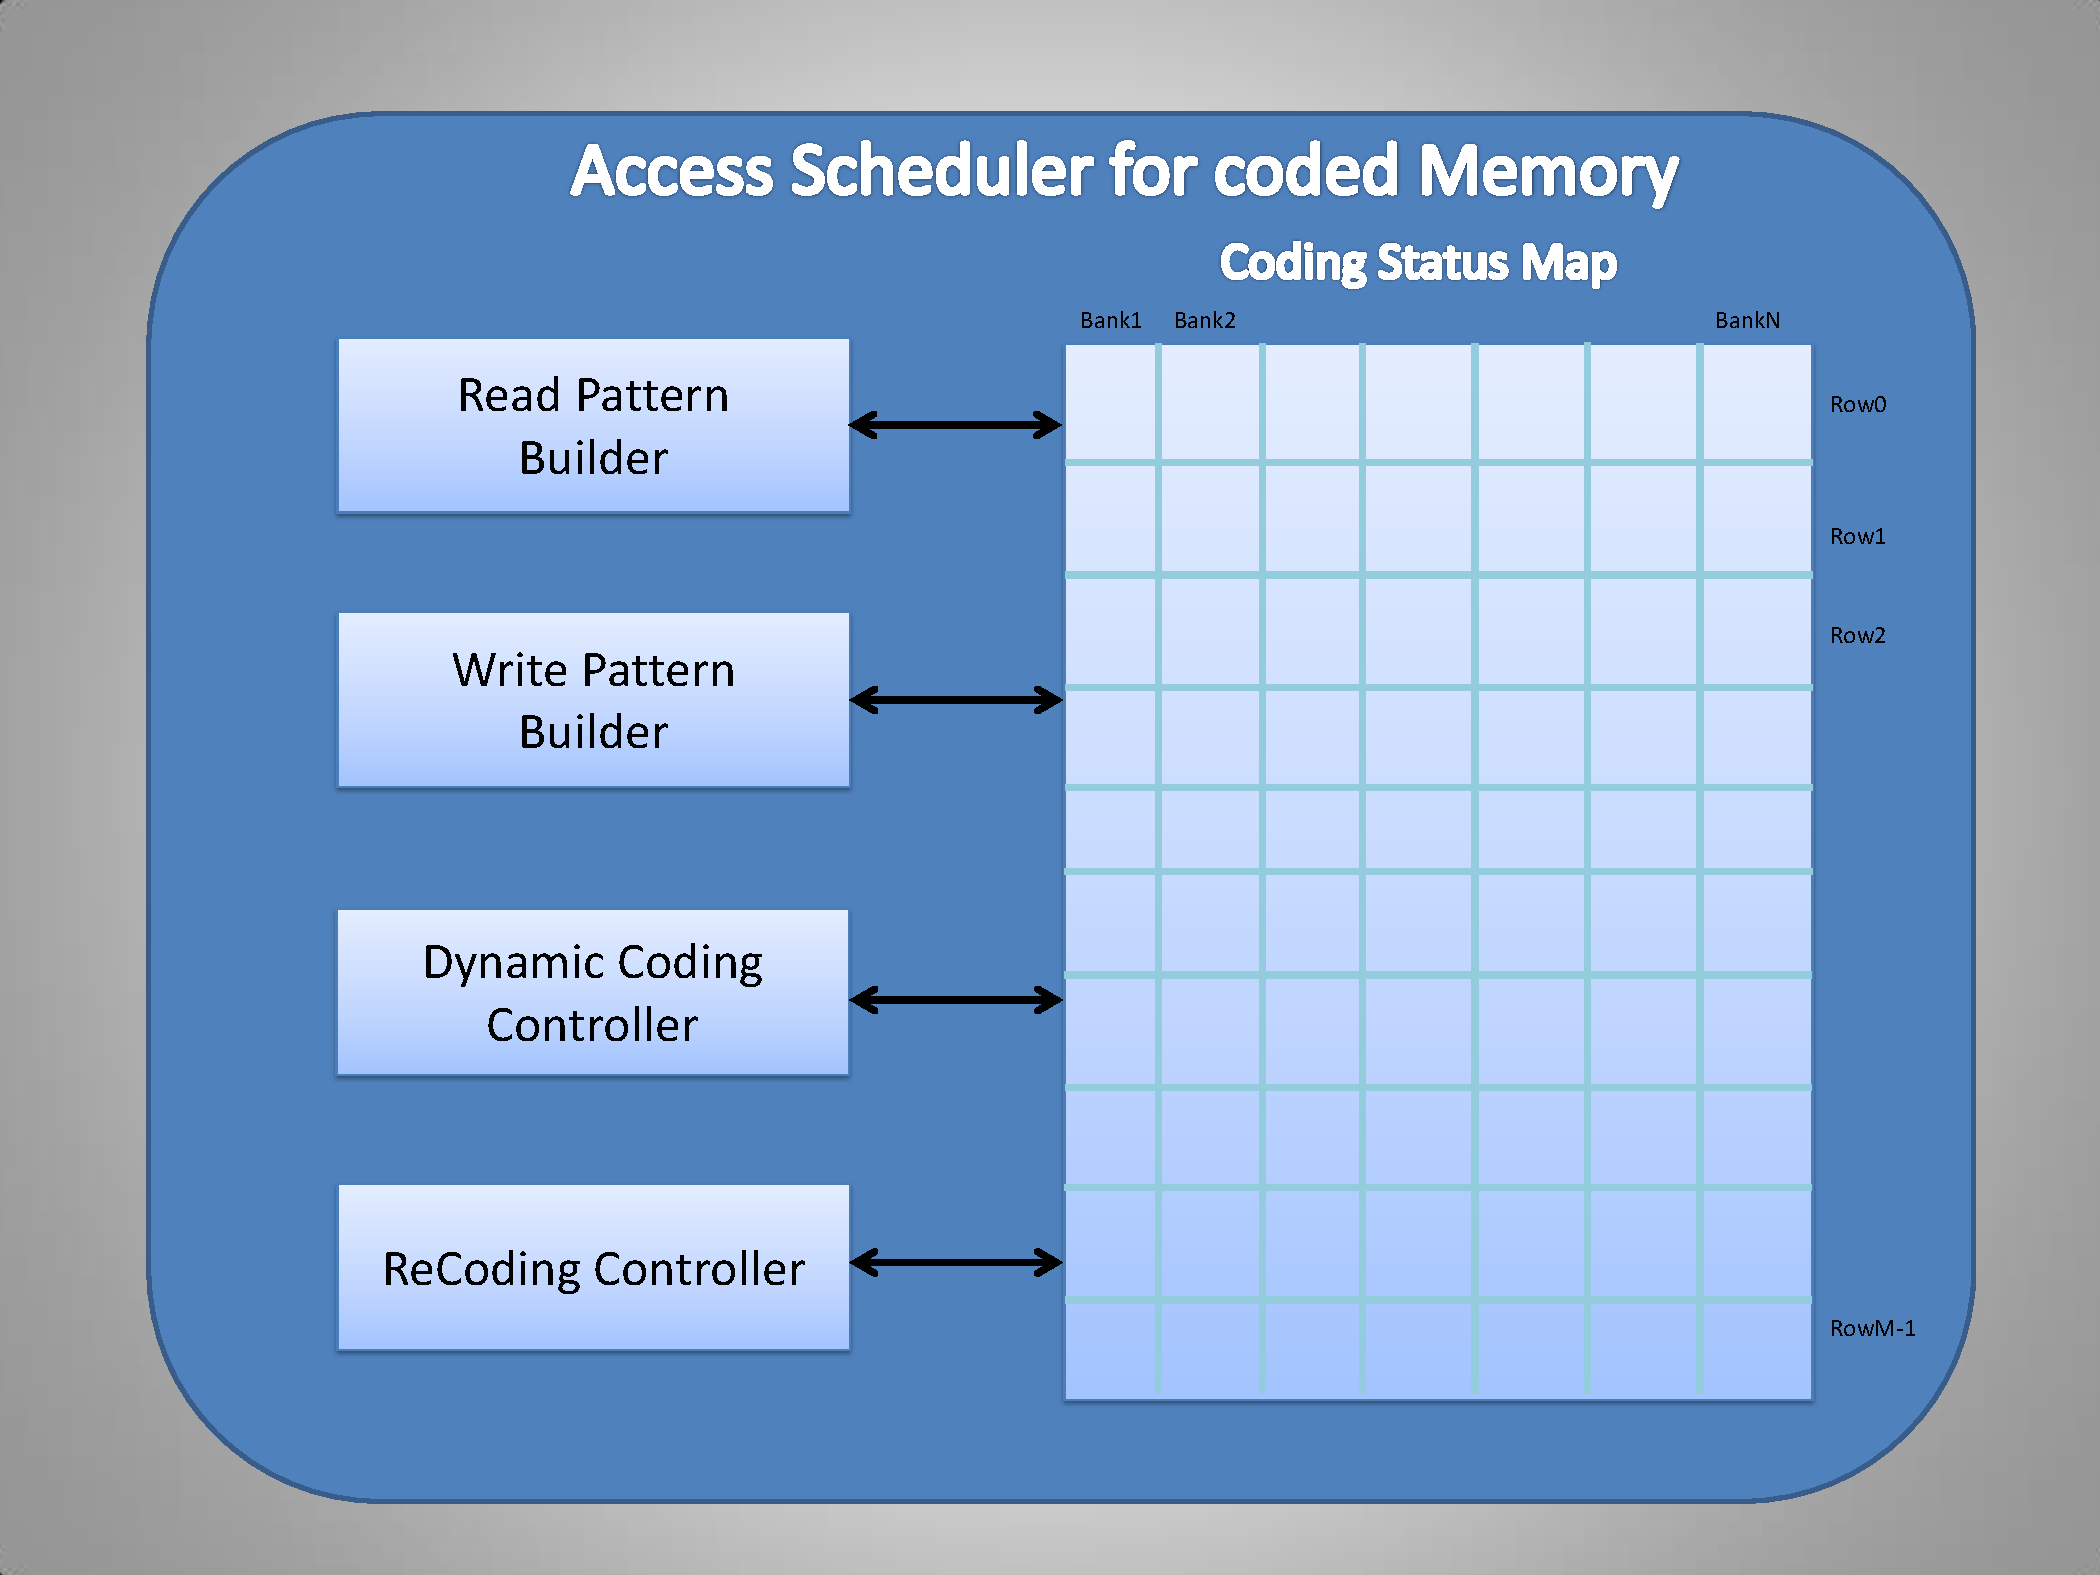
\includegraphics[width=0.7\linewidth]{fig/coded_access_scheduler.pdf}
\caption{
{Access scheduler for coded memory} }
\label{fig:coded_access_scheduler}
\end{figure}
%-------------------------
\subsection{Code Status Table}
\label{sec:codeStatusTable}
The code status table keeps track of the validity of data stored the data and parity banks. The access scheduler may serve a write request using either a data or parity bank. When a write is served to a row in a data bank, any parity bank which is constructed from the data bank will contain invalid data its corresponding row. Similarly, when the access scheduler serves a write to a parity bank, both the data bank which contains the memory address specified by the write request and any parity banks which utilizes that data bank will contain invalid data. The code status table keeps track of the locations of invalid data so the access scheduler does not erroneously serve read requests with stale data.

{\color{blue}
Figure~\ref{fig:coded_access_scheduler} depicts one implementation of the code status table. This is the implementation used to generate the simulation results described in sections 5 and 6. The implementation contains an entry for every row in each data bank. Each entry can take one of three values. The values indicate that either the data in both the data bank and parity banks is fresh, the data bank contains the most recent data, or one of the parity banks contains the most recent data. It is not necessary for the code status table to know which parity bank a write request was served, because the dynamic coding unit described later in this section keeps track of this information. We assume that the elements of the code status table are accessible at a very fast rate. 
}

{\color{red}
This implementation of the code status table can be improved. This code status table does not keep track of the intermediate steps the access scheduler takes when rebuilding codes after a write is served. When rebuilding the memory in two parity banks after a data bank has been written to, it is likely that elements of one parity bank will be restored before the other. The restored parity bank is ready to serve more memory requests using the rebuilt row, but the code status table will indicate that all the parity banks are unavailable until all parity banks are restored. Full knowledge of the status of all data and parity banks allows the access scheduler to serve more requests in some scenarios. \Matt{is this example necessary? Is the tangent worth the insight?}
}

%-----------------------
\begin{figure}[t!]
	%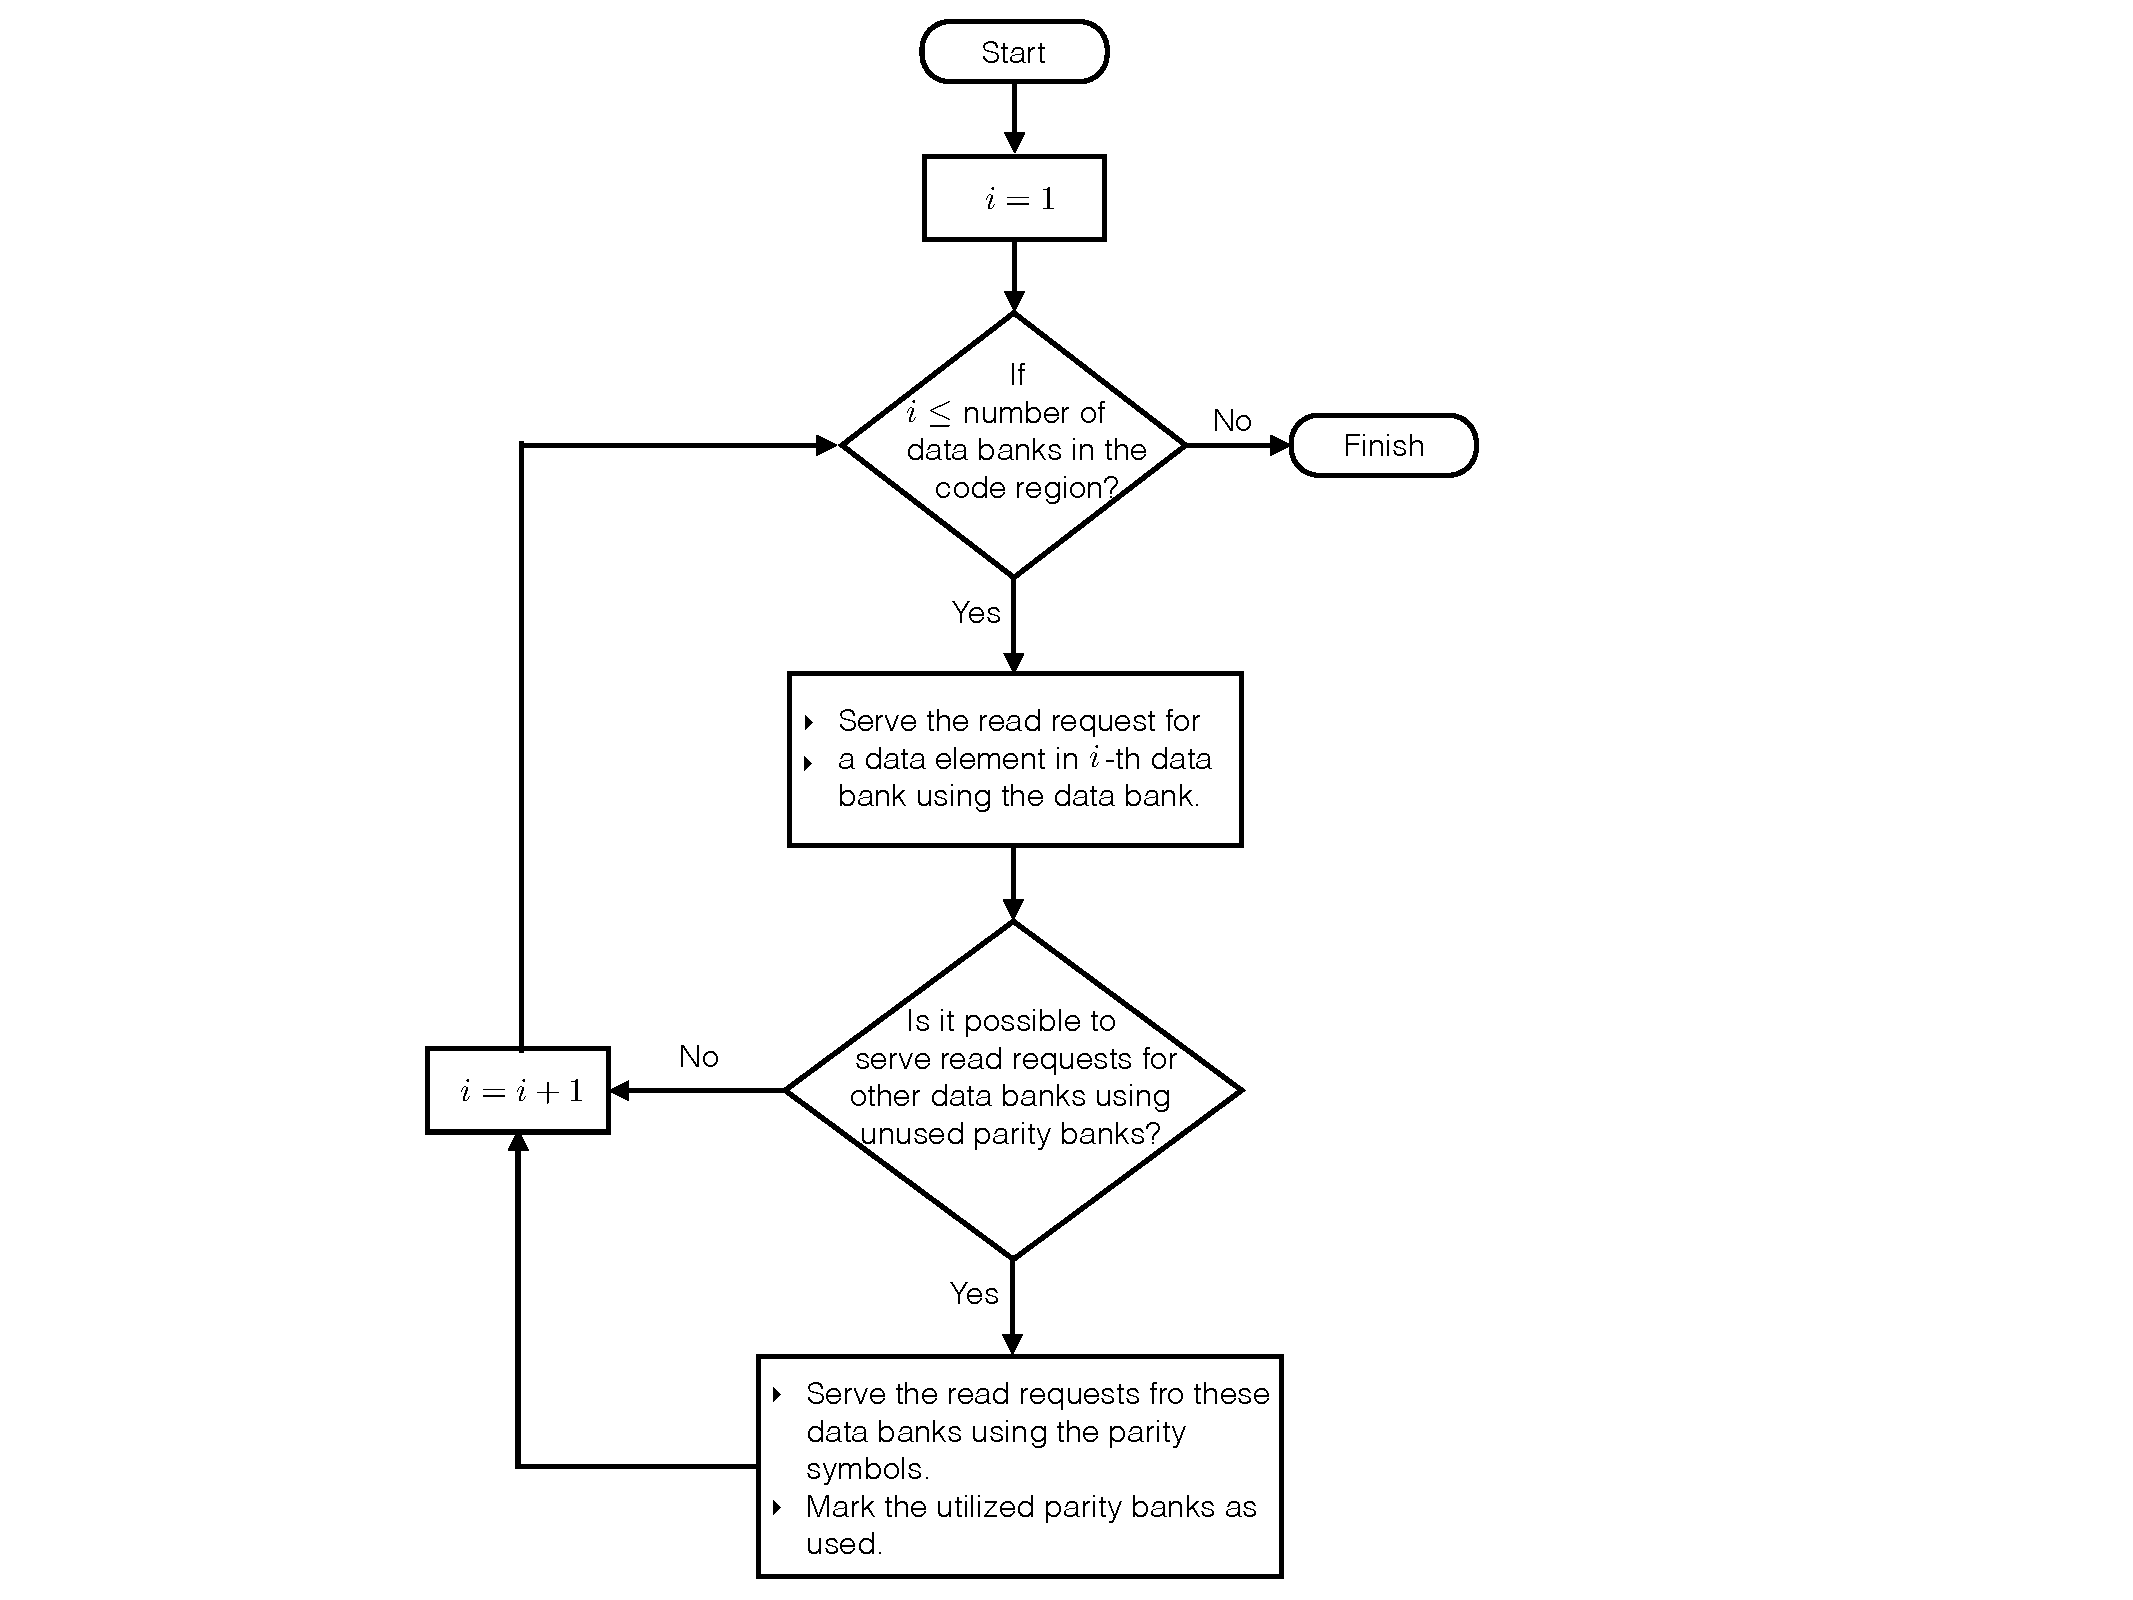
\includegraphics[width=0.9\linewidth]{fig/Read-algo.pdf}
	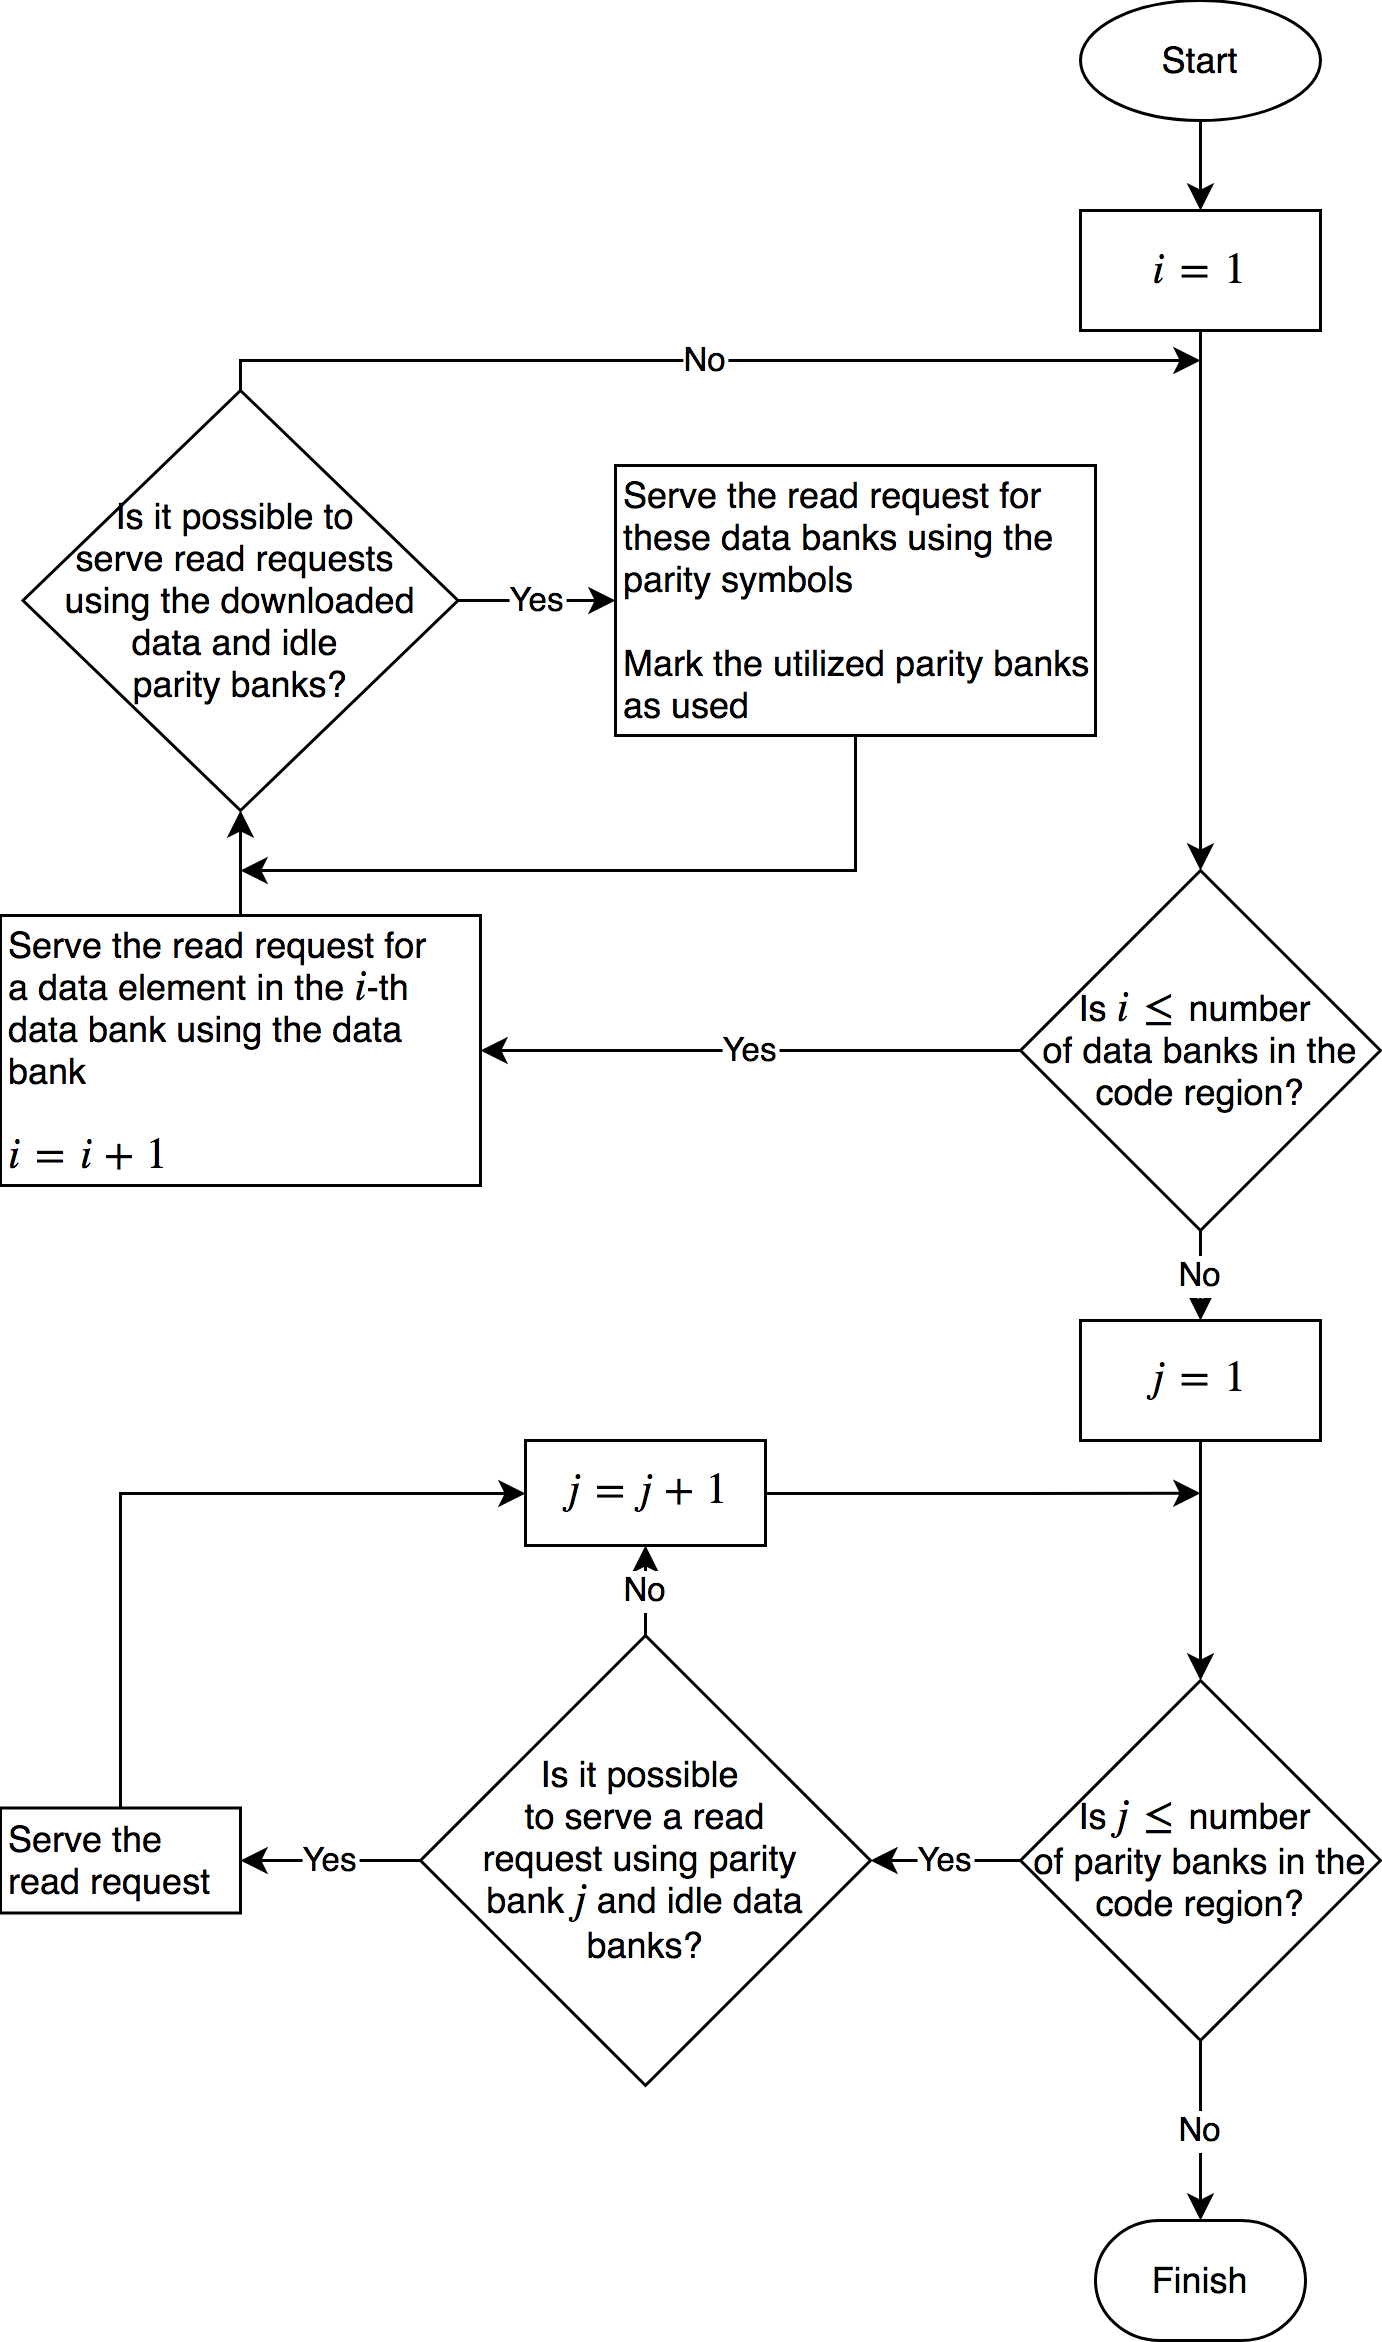
\includegraphics[width=0.96\linewidth]{fig/read_pattern_algo.png}
	\caption{{Description of the algorithm to build a read request pattern to be served in a given memory cycle.}}
	\label{fig:readAlgo}
\end{figure}
%-------------------------
%-----------------------
\begin{figure}[htbp]
	\centering
	%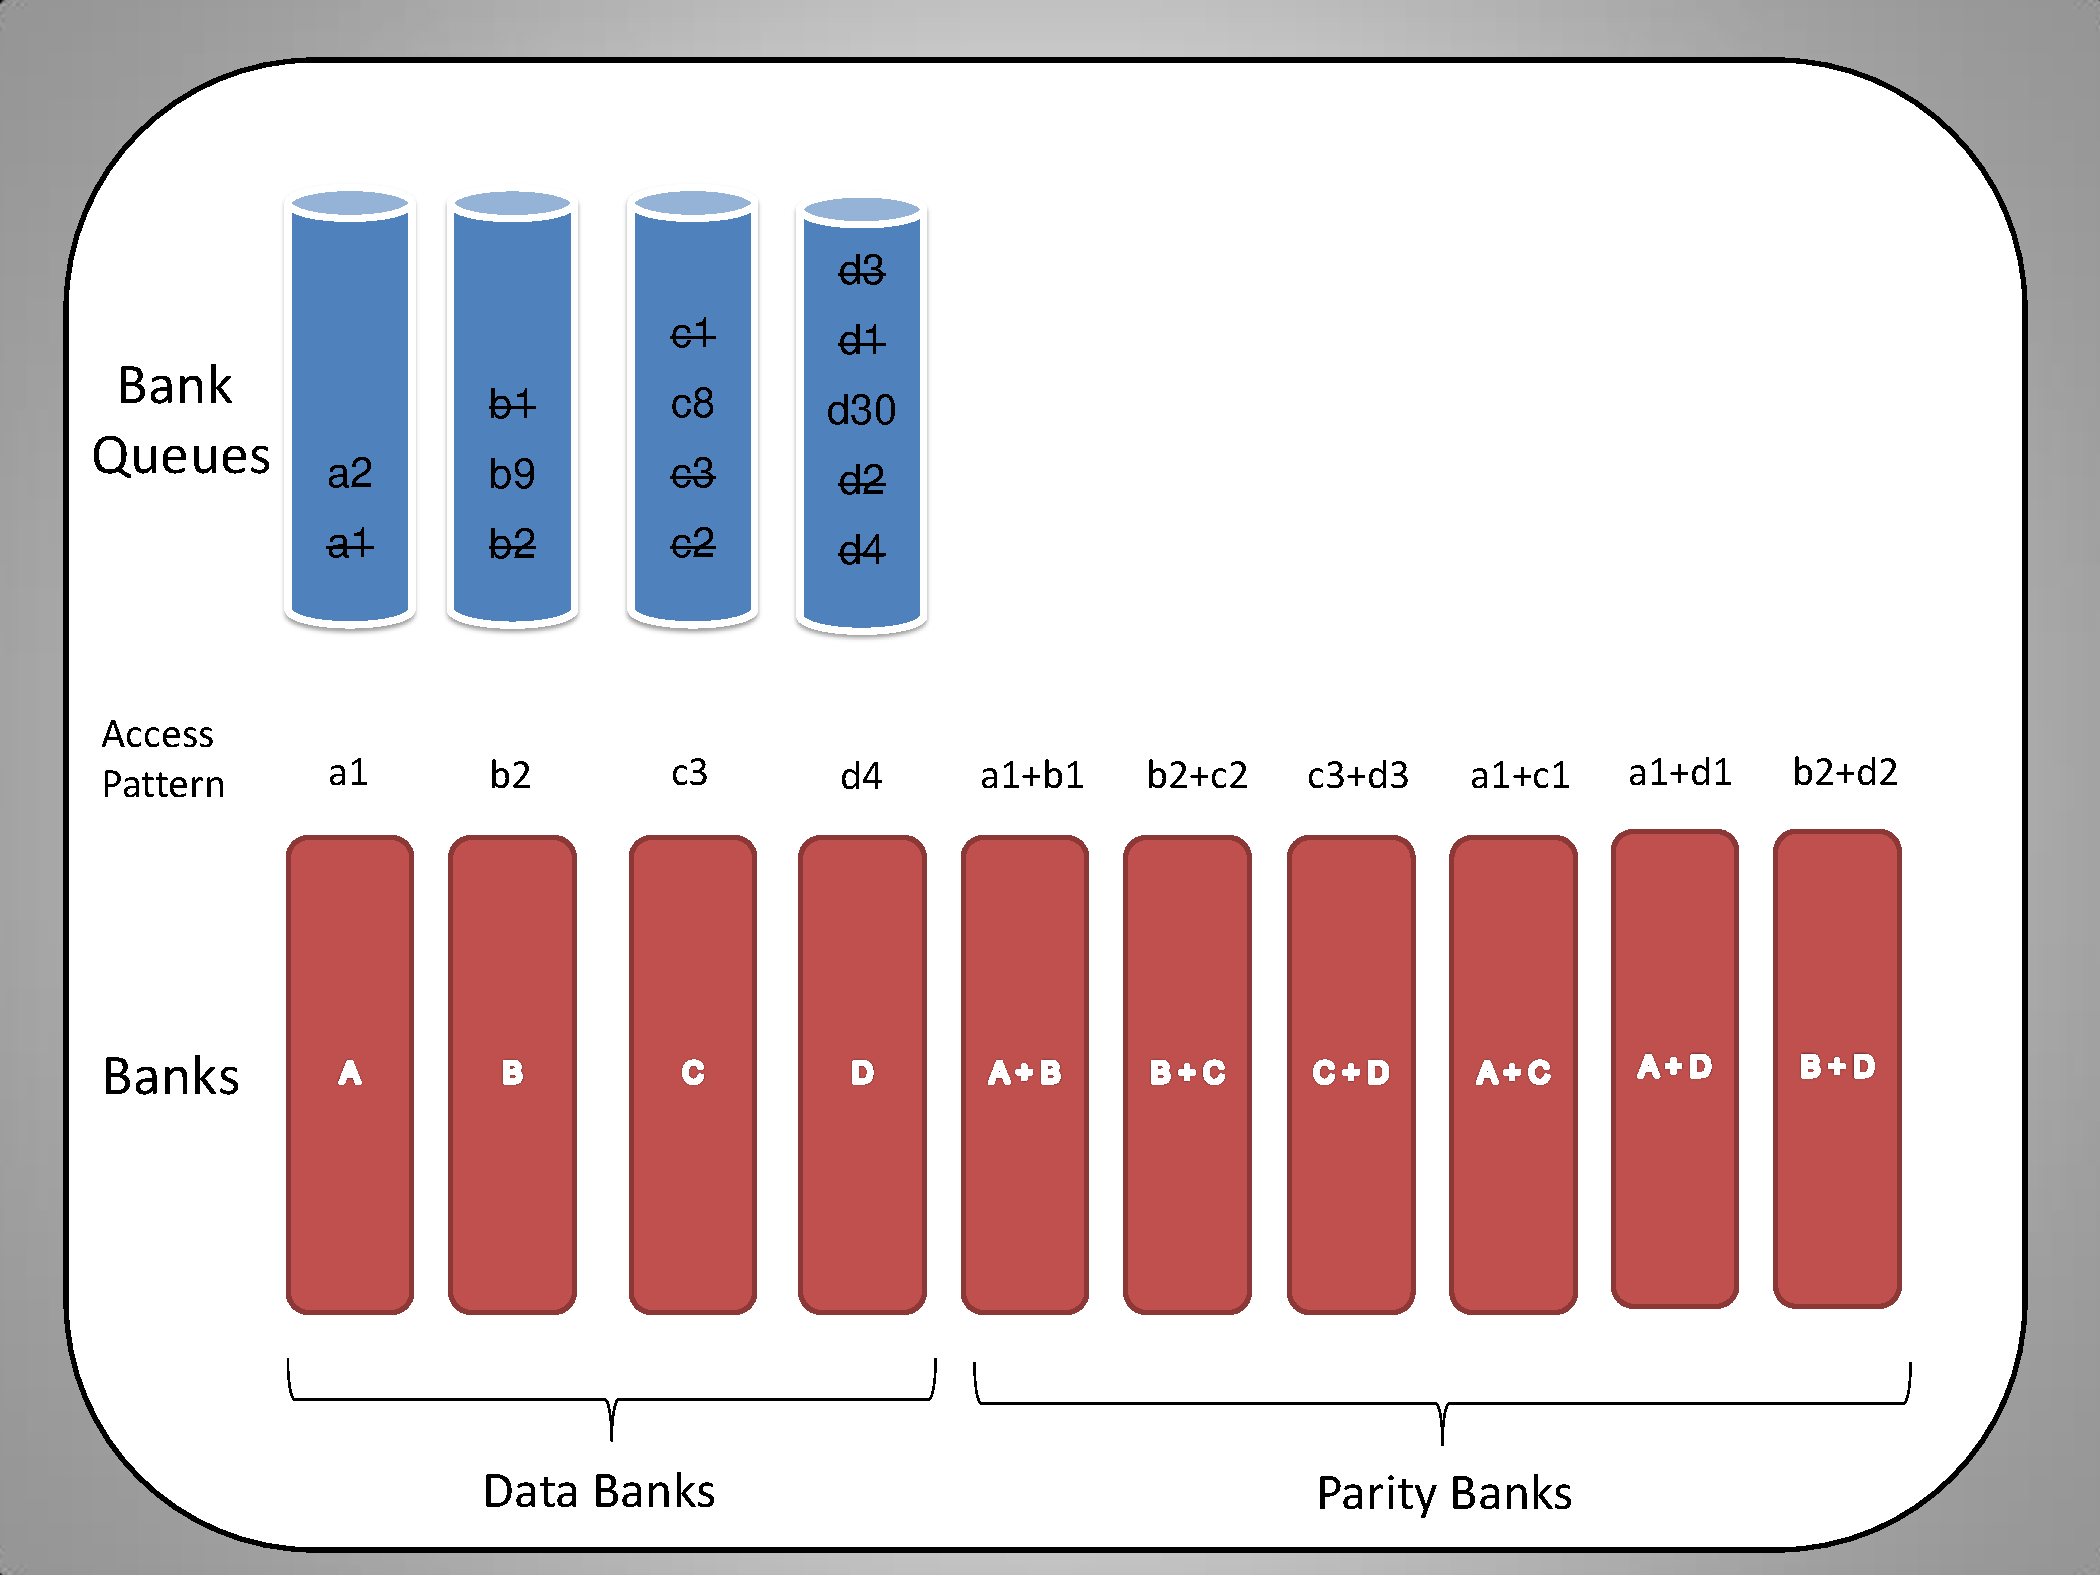
\includegraphics[width=0.7\linewidth]{fig/readAlgoAccessPattern.pdf}
	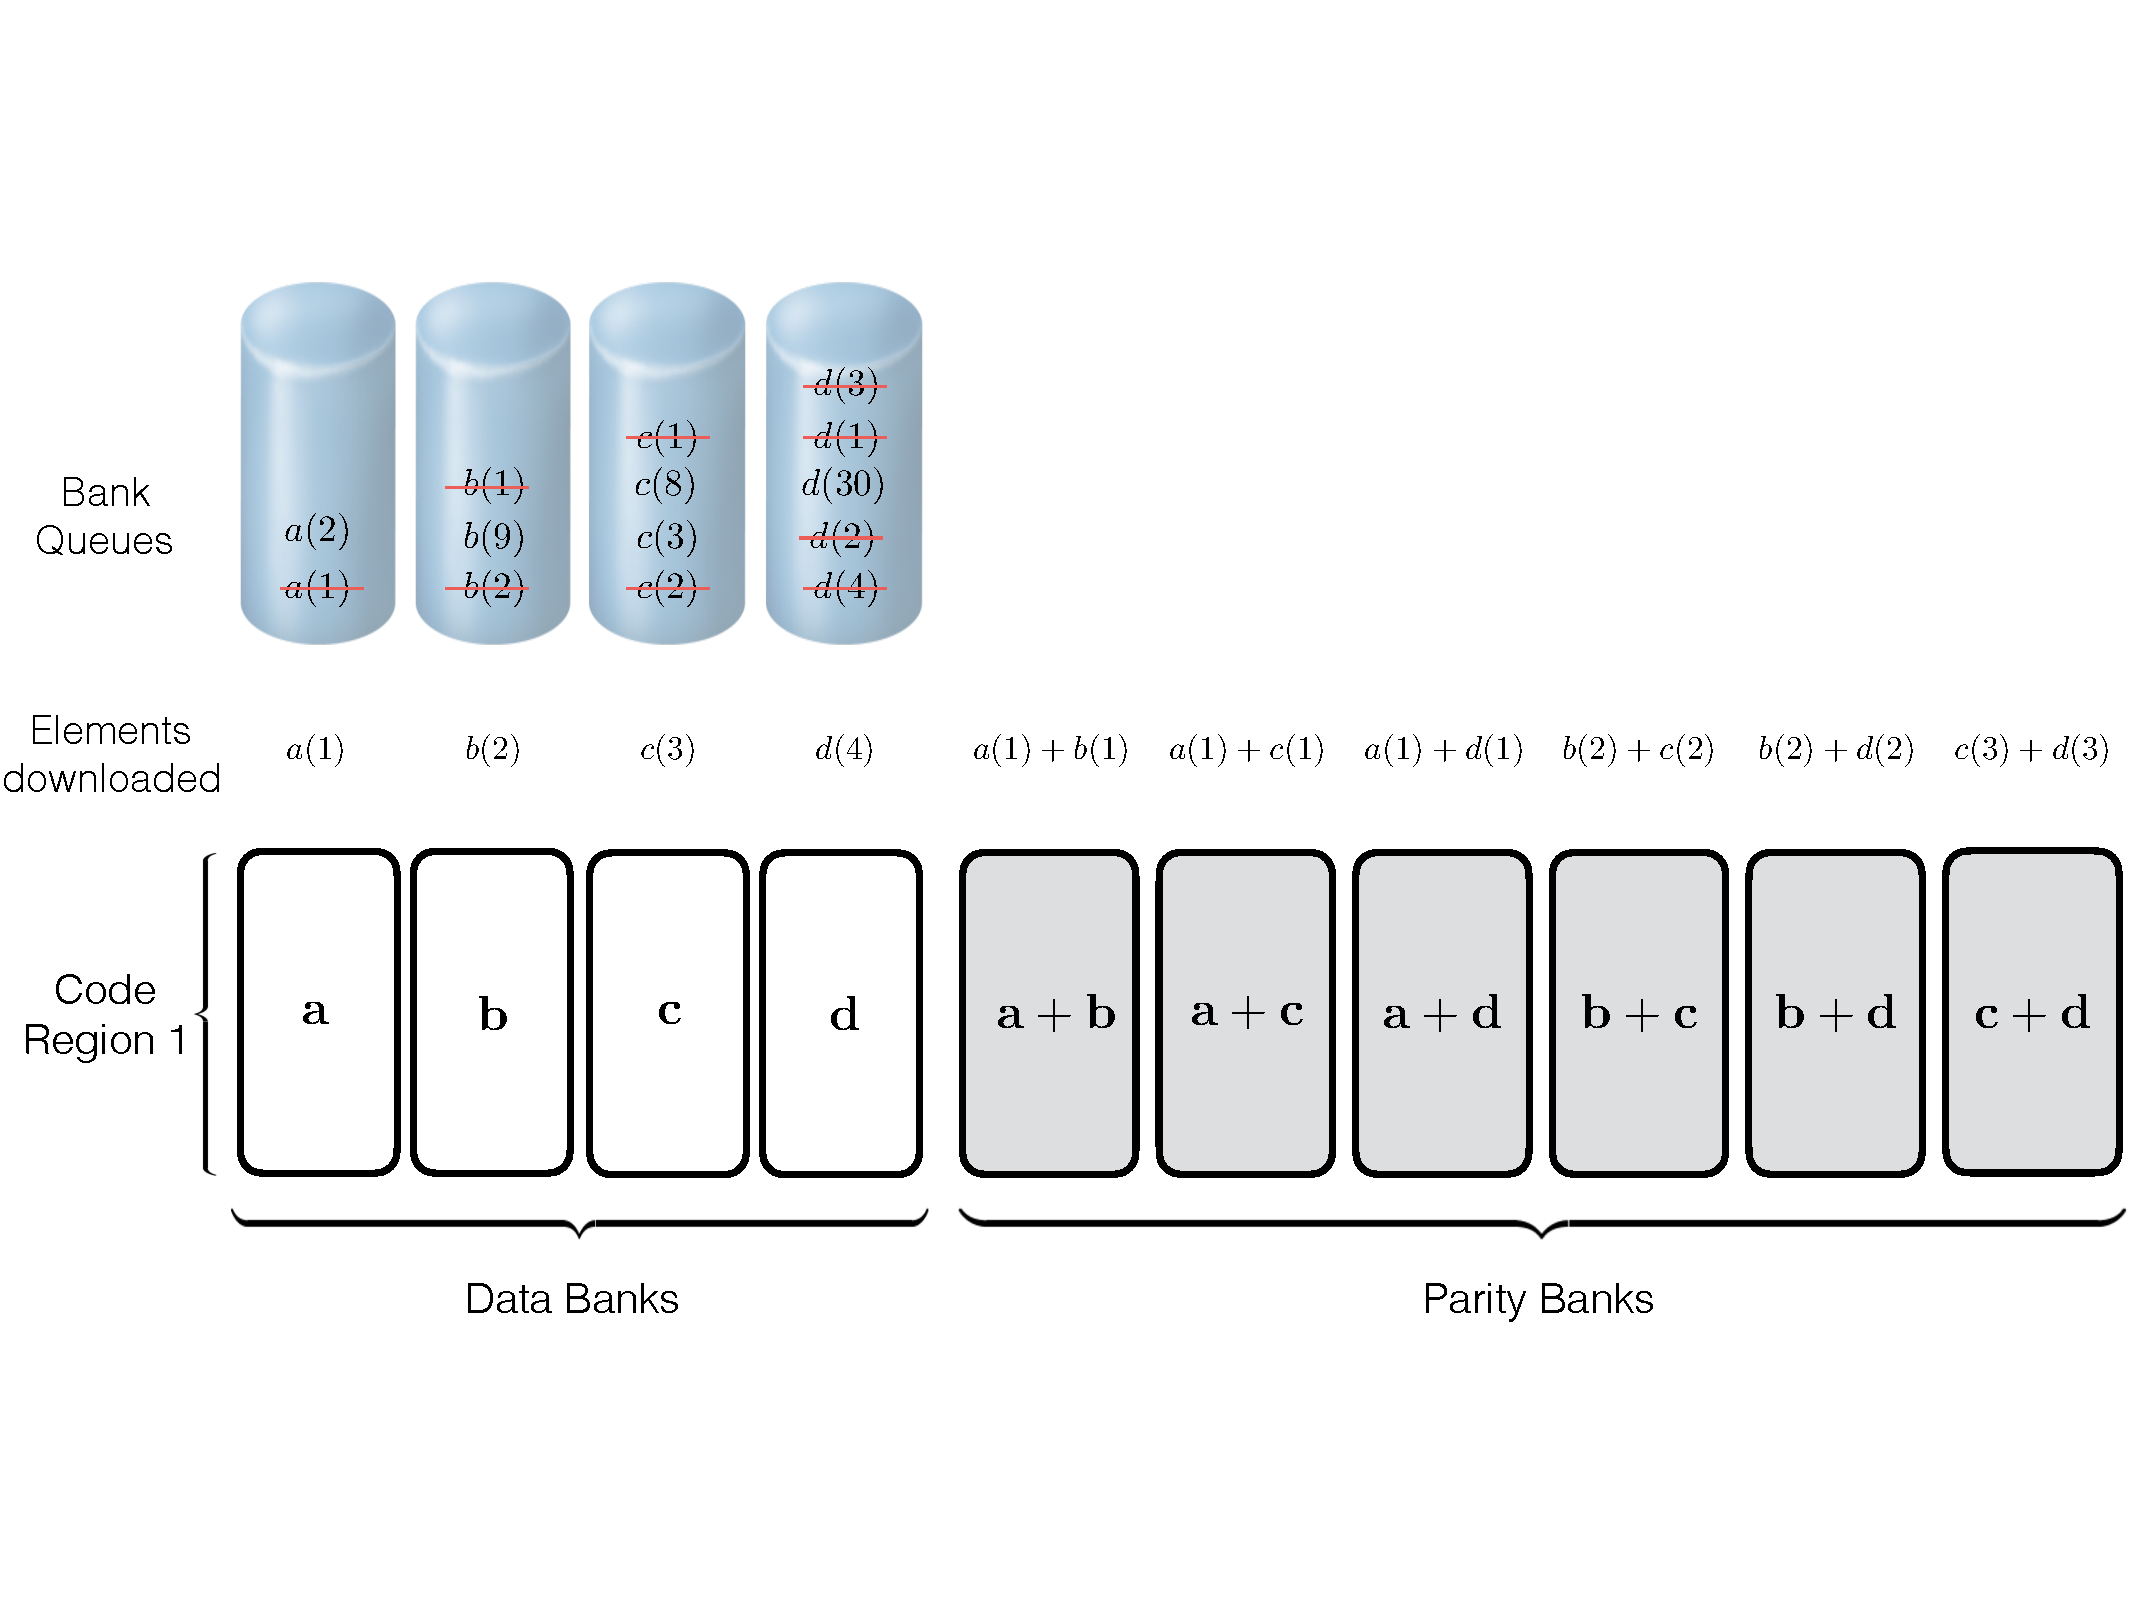
\includegraphics[width=0.96\linewidth]{fig/Read-Algo-Example.pdf}
	\caption{{Illustration of the algorithm to build a read request pattern to be served in a given memory cycle. All the read requests associated with the strikethrough elements are scheduled to be served in a given memory cycle. The figure also shows the elements downloaded from all the memory banks in order to serve these read requests.}}
	\label{fig:readAlgoAccessPattern}
\end{figure}
%------------------------
%\subsection{Read Algorithm for Coded Memory system}
\subsection{Read pattern builder}
\label{sec:readCodingAlgo}

{\color{blue}
A principal goal of the proposed memory system is to serve many read requests in a single memory cycle, and the redundant memory provided by the parity banks gives the memory controller the potential to fulfill this goal. The access scheduler must determine how to use the memory provided by the parity banks. When serving read requests, the access scheduler selects a set of requests to be scheduled from the bank queues. In order to select the set of requests to be scheduled, the access scheduler must determine how the memory requests will be served by the data and parity banks. Serving a memory request from a data bank is straightforward, because the symbols in the data banks uncoded, so they are ready to be used as long as the code status table indicates that the symbols are up-to-date. Serving a memory request using a parity bank more complex, because parity banks which contain coded symbols must use symbols downloaded from data banks in order to be decoded. The access scheduler uses the read pattern builder algorithm to determine which requests to serve using parity and data banks. \Matt{Is this paragraph too wordy?}
}

The read pattern builder selects which memory requests to serve and determines how requests served by parity banks will be decoded. The algorithm is designed to serve many read requests in a single memory cycle. Figure \ref{fig:readAlgo} is one possible implementation of the read pattern builder. It is important to note that the algorithm depicted will not always schedule the maximum number of read requests in a single memory cycle. We use the implementation shown here in our simulations described in sections 5 and 6. 

Figure ~\ref{fig:readAlgoAccessPattern} shows the algorithm depicted in one scenario. First, the read pattern builder marks $a(1)$ to be read from data bank $\mathbf{a}$. It then looks through banks $\mathbf{b}$, $\mathbf{c}$, and $\mathbf{d}$ searching for requests for rows $b(1)$, $c(1)$, or $d(1)$ because these symbols can be decoded from a parity bank using the $a(1)$ symbol. In this scenario $b(1$), $c(1)$, and $d(1)$ are all present in the bank queues and are served using parity banks. Symbols equal to  $a(1) + b(1)$, $a(1) + c(1)$, and $a(1) + d(1)$ are all downloaded from parity banks and decoded with $a(1)$. Next, $b(2$) is read from a data bank. Similar to before, $c(2)$ and $d(2)$ are served by downloading $b(2) + c(2)$ and $b(2) + d(2)$ symbols from the parity banks. Again as before, $c(3)$ is read from data bank and $d(3)$ is decoded using $c(3)$ and $c(3) + d(3)$. Finally, $d(4)$ is read from a data bank. In this scenario, Only the top loop of the read pattern builder as pictured in Figure~\ref{fig:readAlgo} schedules reads, but there are scenarios where the bottom loop is useful. \Matt{I have an optimal algorithm for scheduling read requests. Should I include it in this section?}

\begin{remark}
{\color{blue}
Here we note that the aforementioned approach of maximizing the number of read request being served per cycle does come with a cost. It increases the chances of having out-of-order execution of memory access requests. This does not pose a problem in the case when the memory requests go out of order for different cores. However, in order to prevent the out-of-order execution of the access requests arising from the same core, the logic needs to take care of in-order execution of requests from each cores. We assume that the code arbiter only admits requests into the bank queues if the requests can be immediately served without the risk of out-of-order execution.
}

\end{remark}
\ignore{
%-----------------------
\begin{figure}[htbp]
\centering
	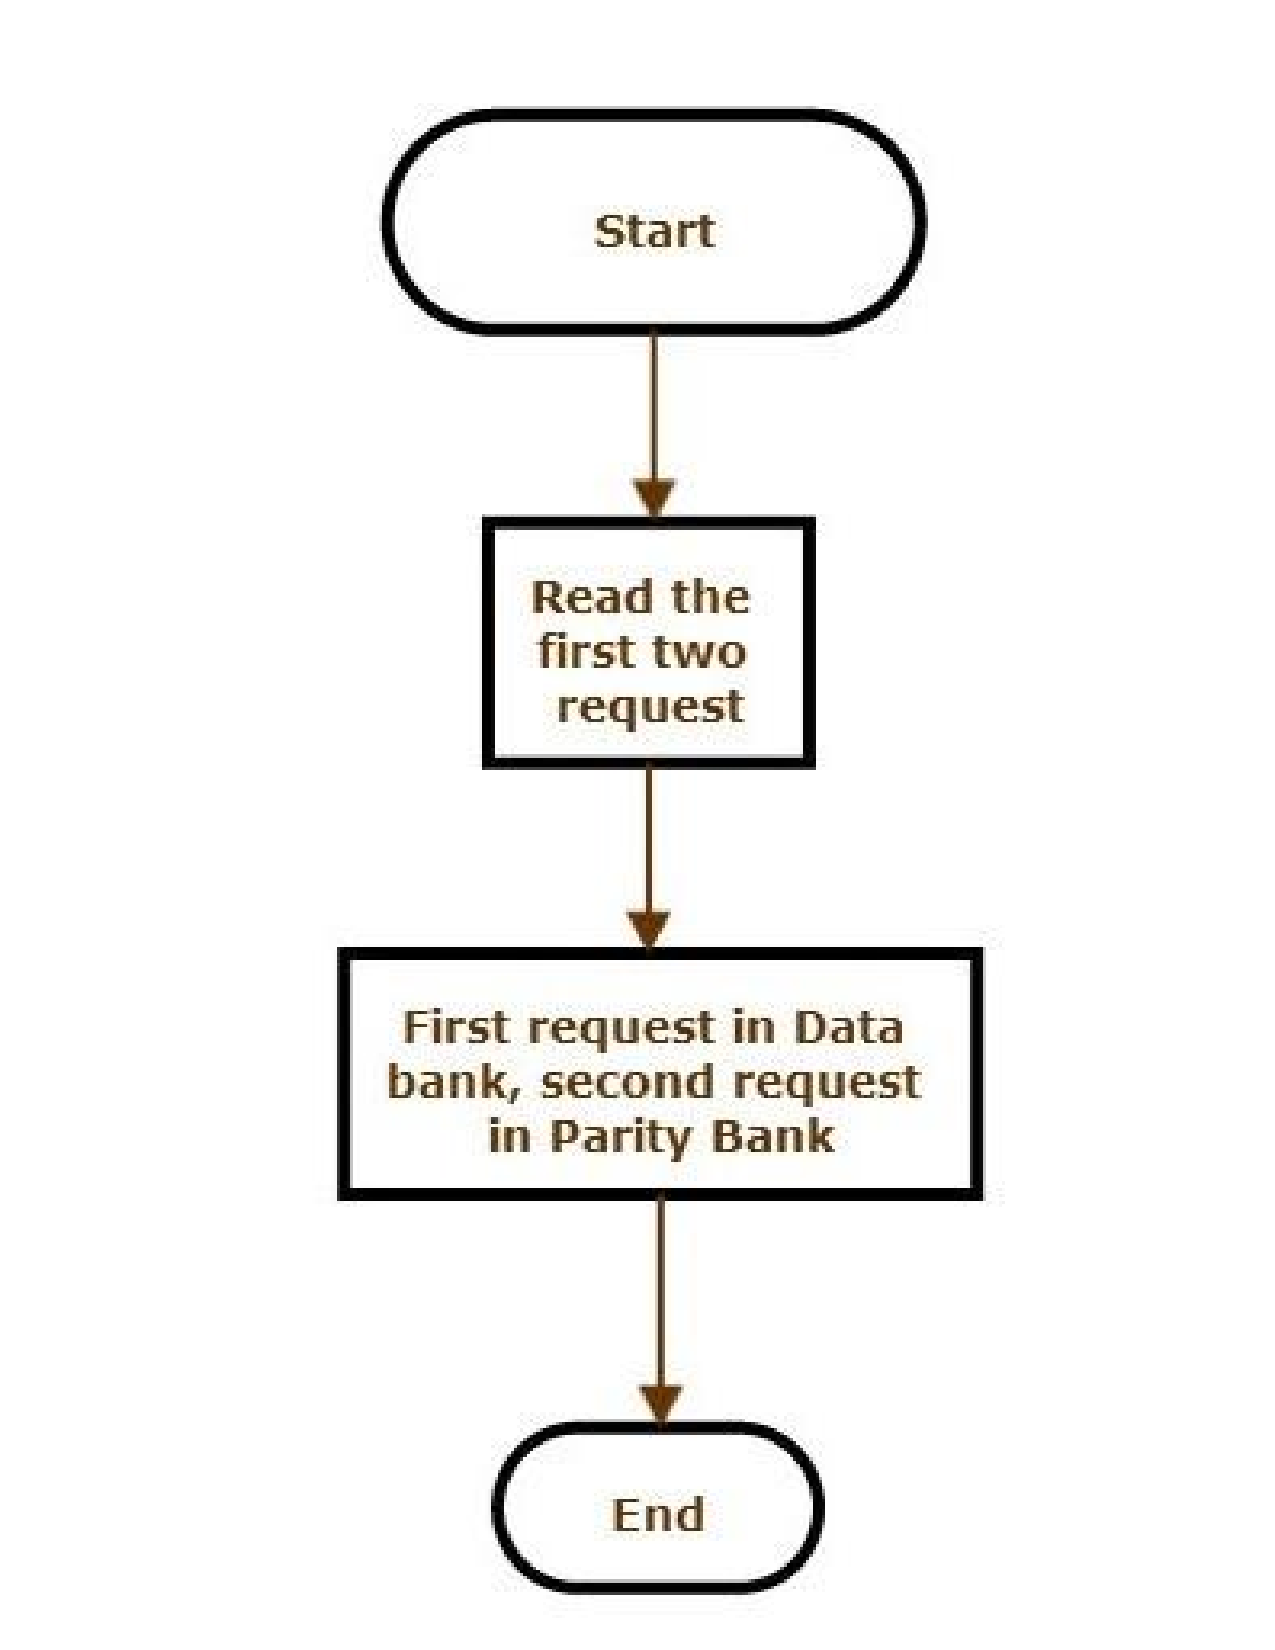
\includegraphics[width=\linewidth]{fig/writealgo.pdf}
	\caption{{\bf Flowchart of Write Algorithm}}
	\label{fig:writeAlgo}
\end{figure}
%-------------------------
%\ignore{
\begin{itemize}
\item Write about how we solve the out of order look ahead problem. If we solve 
	it at all ????
\end{itemize}
}
%\subsection{Write Algorithm for Coded Memory system}
\subsection{Write pattern builder}
\label{sec:writeCodingAlgo}
The inclusion of parity banks allows the memory controller to serve additional write requests per cycle. The memory controller can serve multiple writes which target a single data bank by committing some of the writes to parity banks. Similar to the read pattern builder, the access scheduler implements a write pattern builder algorithm which determines which write requests to schedule in a single memory cycle. 

%-----------------------
\begin{figure}[htbp]
\centering
	\includegraphics[width=\linewidth]{fig/write_pattern_algo.png}
	\caption{{ Flowchart of write pattern builder}}
	\label{fig:writeFlow}
\end{figure}
%-------------------------

Figure~\ref{fig:writeFlow} illustrates a potential implementation of the write pattern builder. The implementation of the write pattern builder discussed here is used in the simulations described in sections 5 and 6. Only when the write bank queues are nearly full does the access scheduler execute the write pattern builder algorithm. 

Figure~\ref{fig:writeAlgoAccessPattern} shows how the write pattern builder described in Figure~\ref{fig:writeFlow} performs in one scenario. Without the parity banks only one write request can be scheduled for each of the four data banks. The inclusion of parity banks allows for 10 write requests to be scheduled. Note that an element which is addressed to row $n$ in a data bank can only be written to the corresponding row $n$ in the parity banks. In this scenario, the write queues for each data bank are full. The controller takes $2$ write requests from each queue and schedules one to be written to their target data bank the other to a parity bank. The controller also updates the code status table. \Matt{The figure figure here contains an error - 10 write requests should be served}

{\color{red}
Figure~\ref{fig:writeAlgoAccessPattern} also demonstrates how the code status table changes to reflect the freshness of the elements in the data and parity banks. Here, the 00 status indicates that all elements are updated. The 01 status indicates that the data banks contain fresh elements and the elements in the parity banks must be recoded. The 10 status indicates that the parity banks contain fresh elements, and that the data bank must be updated and the elements in the parity banks must be updated.
}

%-----------------------
\begin{figure}[t!]
\centering
         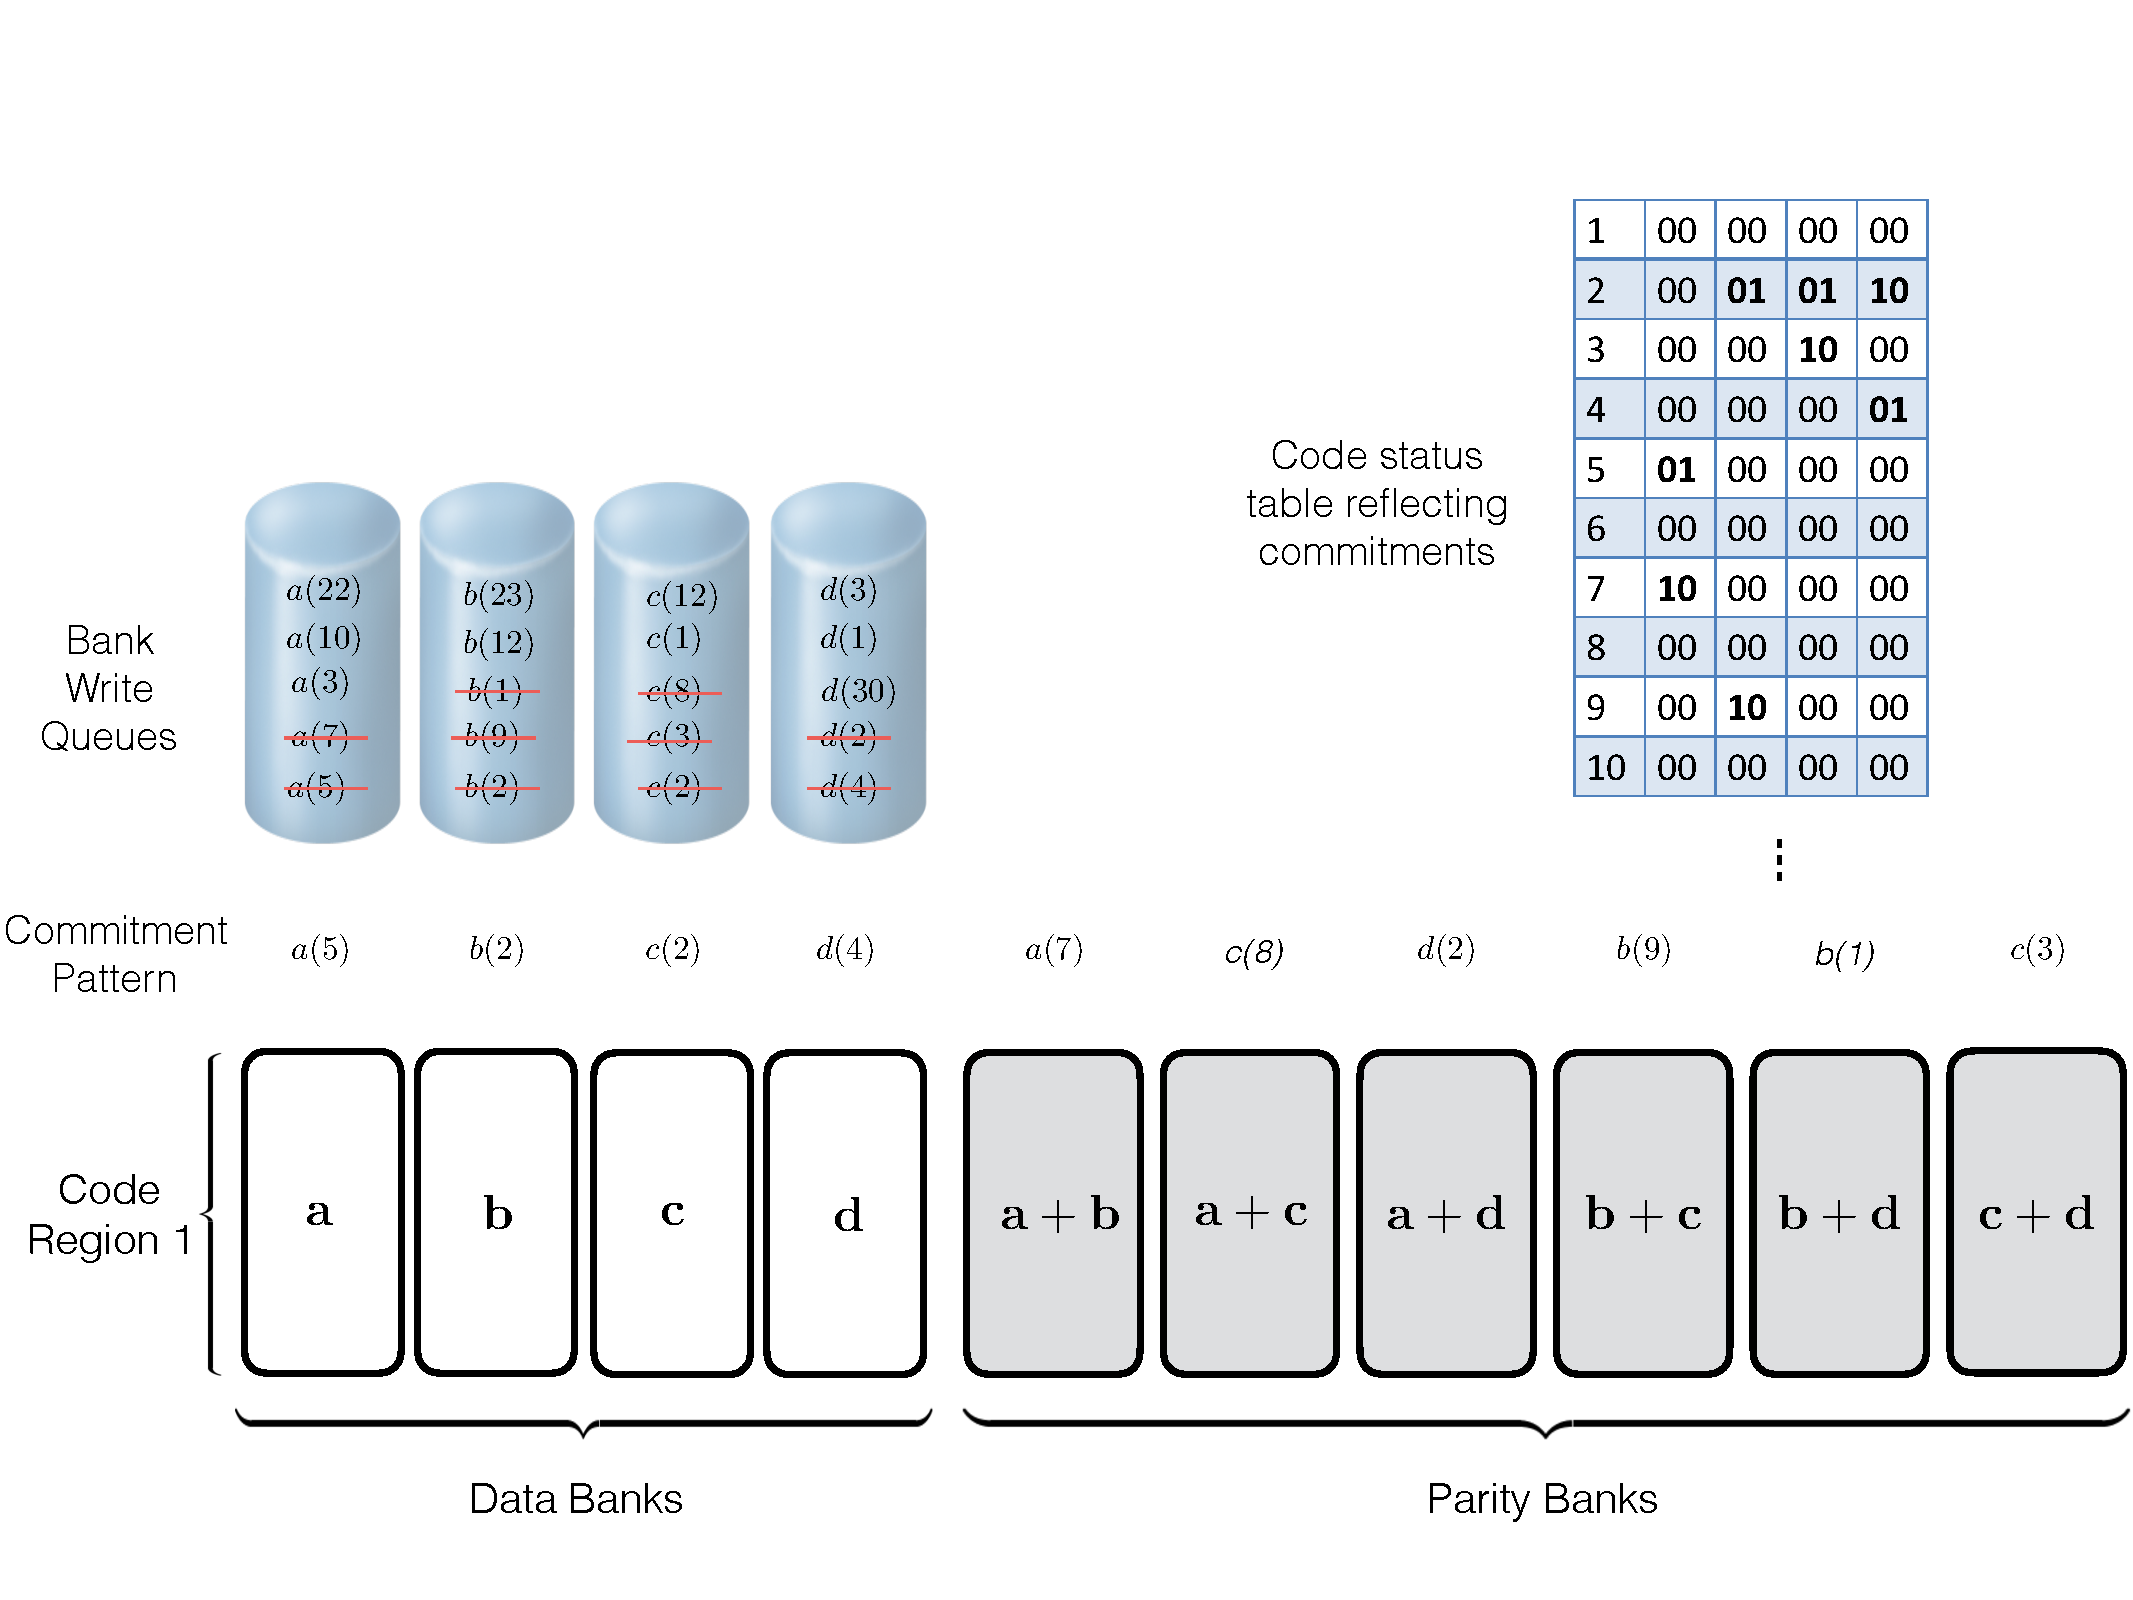
\includegraphics[width=\linewidth]{fig/Write-Algo-Example.pdf}
	\caption{Figure describing write algorithm access pattern}
	\label{fig:writeAlgoAccessPattern}
\end{figure}
%-------------------------
\subsection{ReCoding unit}
\label{sec:recoding}
After a write request has been served, the stale data in the parity or data banks must be replaced. The ReCoding Unit is responsible for updating the elements of data and parity banks after a write is served. The ReCoding Unit contains a queue of {\em recoding requests}. Every time a write is served, recoding requests are pushed on to the queue. Recoding requests indicate which data and parity banks contain stale elements, and they indicate the bank the write was served to which generated the recoding request. The recoding requests also contain the cycle number the request was created so the ReCoding Unit may prioritize older requests. 

\subsection{Dynamic Coding}
\label{sec:dynamicCoding}
To reduce memory overhead, the size of the parity banks is designed to be only a fraction of the size of the data banks. Ideally, the most heavily accessed portions of memory are stored in the parity banks. The dynamic coding block is responsible for maintaining codes for the most heavily accessed memory sub regions.

\subsubsection{Motivation}
Bank conflicts are most likely to occur when regions of shared-memory are localized to certain memory regions. Multi-core systems often generate memory access requests to overlapping memory regions. By dynamically coding certain memory locales, the proposed memory system aim to resolve the bank conflicts which occur during periods of heavy memory access in multi-core systems.

\begin{figure}[htbp]
		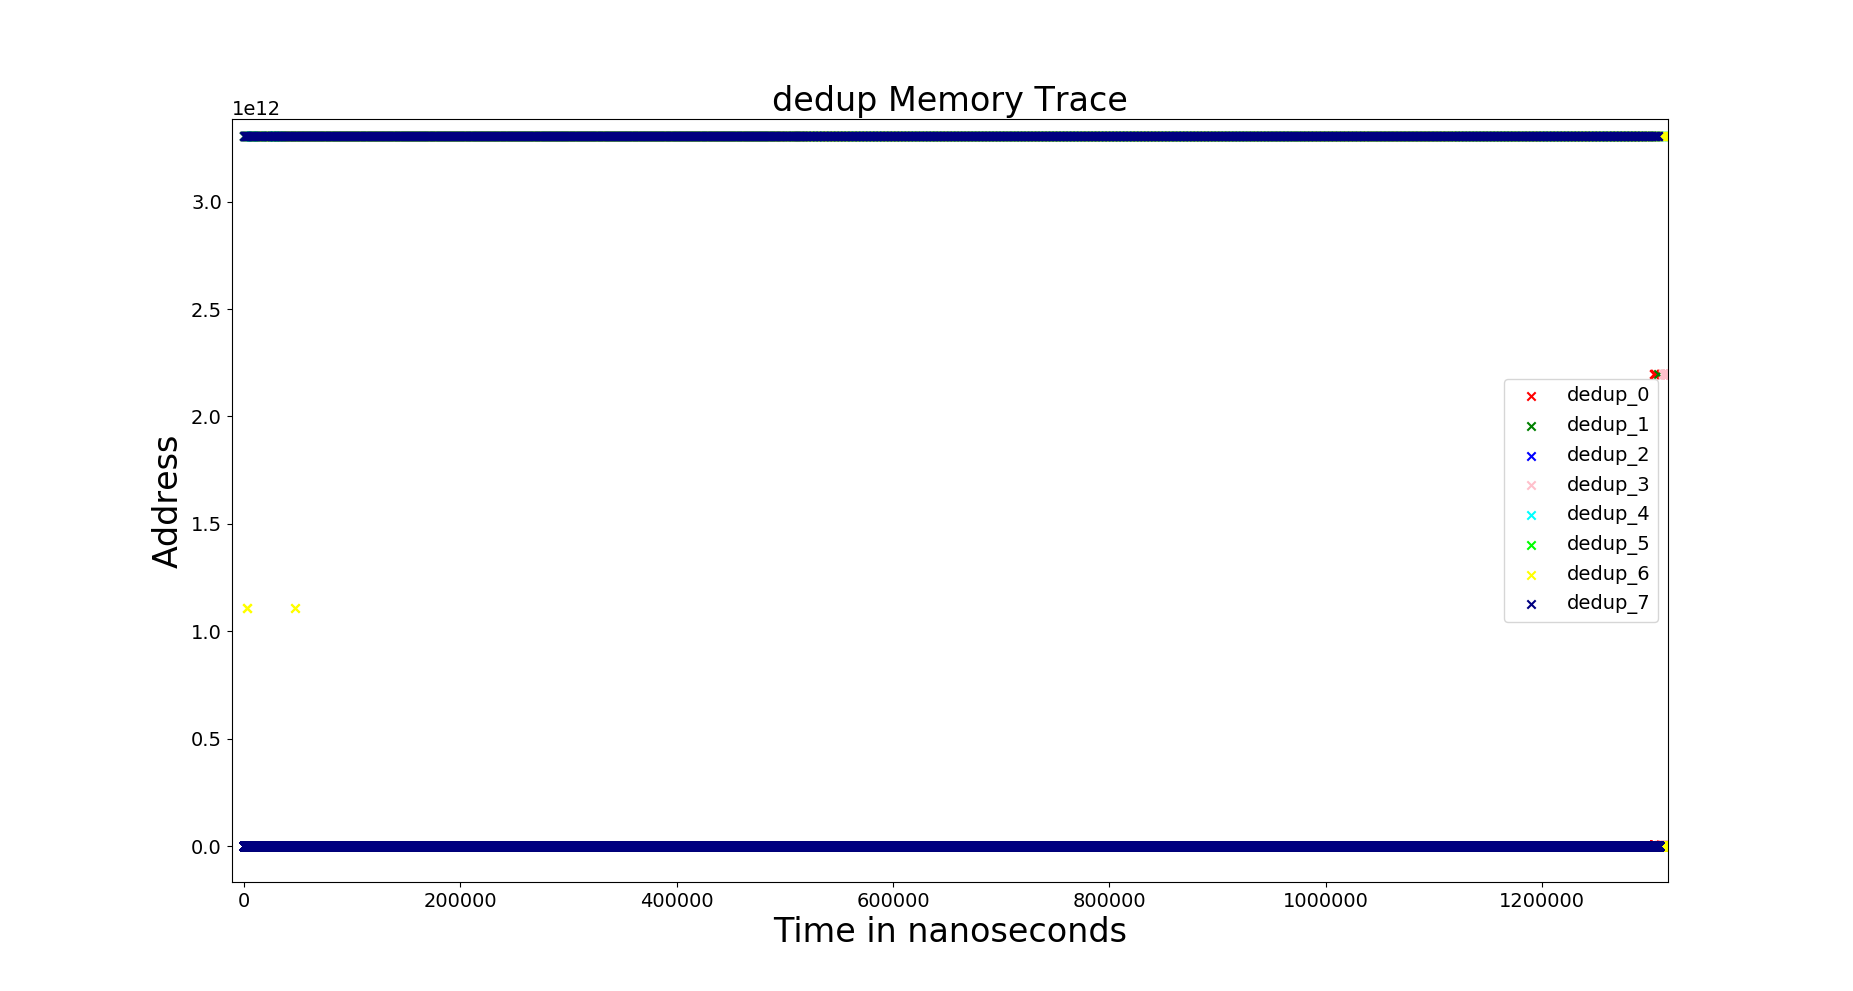
\includegraphics[width=\linewidth]{fig/dedup_whole.png}
		\caption{Memory Access from the Dedup PARSEC benchmark. This trace was generated using 8 cores.}
		\label{fig:dedup_whole}
\end{figure}

\begin{figure}[htbp]
		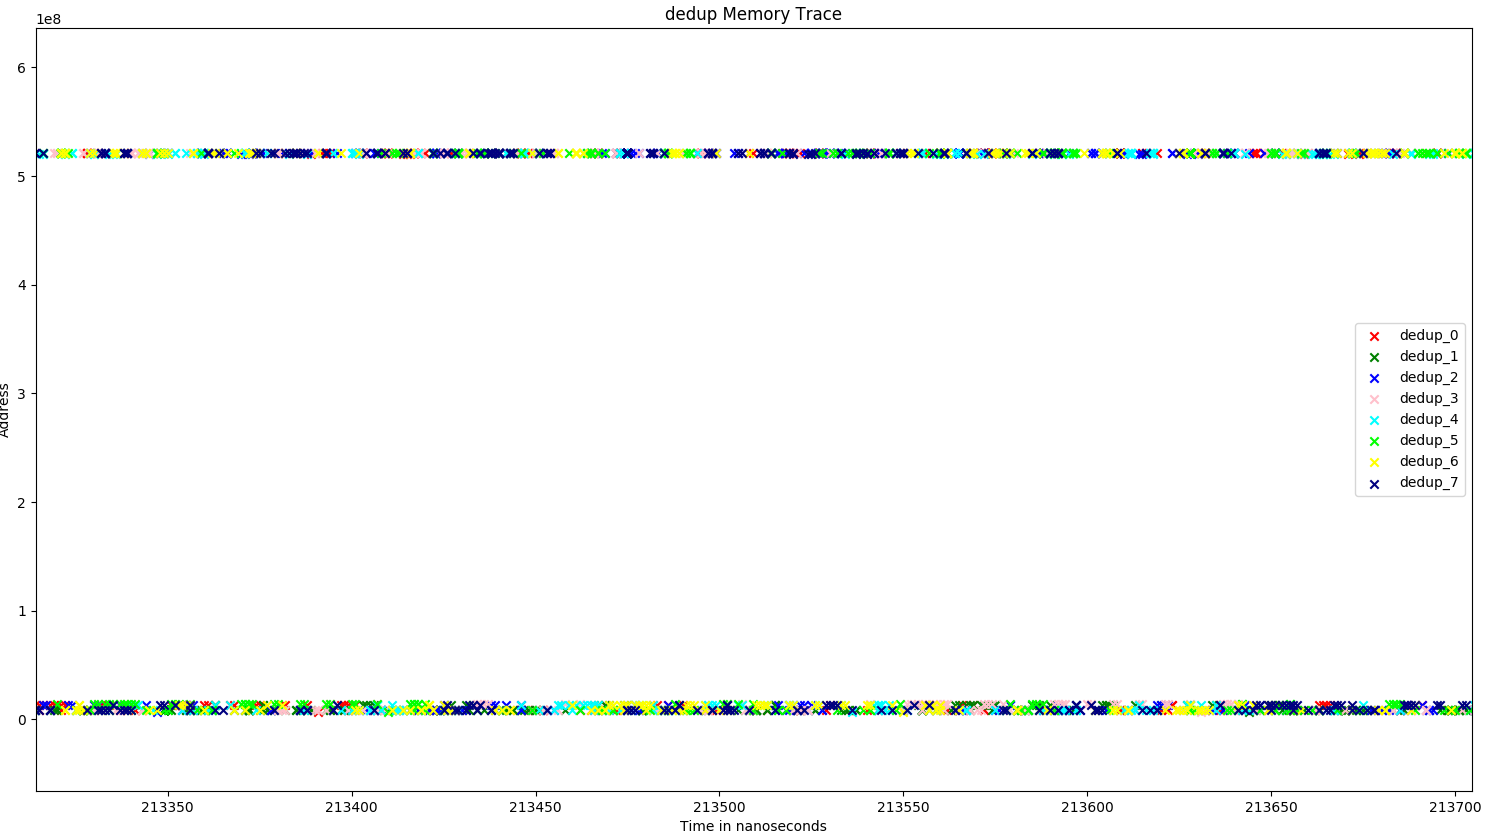
\includegraphics[width=\linewidth]{fig/dedup_dense.png}
		\caption{Memory Access from the Dedup PARSEC benchmark demonstrating the density of memory accesses}
		\label{fig:dedup_dense}
\end{figure}

An examination of the memory trace from one of the PARSEC benchmarks illustrates a scenario where dynamic coding works well. Figure~\ref{fig:dedup_whole} shows the memory trace of a simulation of an 8-core system running the dedup PARSEC benchmark. The y-axis shows the address accessed by the cores. The x-axis shows the access time in nanoseconds. This plot shows that most of the accesses from various cores are primarily located in the lower memory band. Greater than 95\% of all memory accesses are in this band. Figure~\ref{fig:dedup_dense} magnifies this band and reveals that the lower band is composed of two sub-bands of roughly equal density. In a scenario where the dynamic coder can choose to encode two memory blocks it would  would detect that nearly all memory access are localized to the primary memory bands, so only those regions would be encoded.

\subsubsection{Encoder Design}
There are many possible implementations of the dynamic coding unit. The design described here is used in the simulator used to generate the results described in sections 5 and 6.

The {\em dynamic coding} block splits the each memory bank according to the memory partition coefficient {\em r}. Each bank is split into $\lceil\frac{1}{r}\rceil$ partitions. Recall that $\alpha$ is the maximum memory overhead of the proposed memory system. The block can select up to $\frac{\alpha}{r} - 1$ regions to be encoded in the parity banks. A single region is reserved to allow the dynamic coding block to encode a new region.

Every $T$ ticks, the {\em dynamic coding} unit chooses the $\frac{\alpha}{r} - 1$ regions with the greatest number of memory accesses. The dynamic coding unit will then encode these regions in the parity banks. If all the selected regions are already encoded, the unit does nothing. Otherwise, the unit begins encoding the most accessed region. Once the dynamic coding unit is finished encoding a new region, the region becomes available for use by the rest of the memory controller. If the memory ceiling $\alpha - r$ is reached when a new memory region is encoded, the unit evicts the least frequently used encoded region.

{\color{blue}
\subsection{Prefetching Codes}
\label{sec:prefetching}
Dynamic coding works best when the most heavily accessed regions of memory do not change over time. Though dynamic coding can still be effective when the memory access trend is not static, the proposed memory system can benefit from a system which anticipates sequential memory accesses. 
The prefetcher attempts to detect sequential memory accesses and exploit idle memory banks to potentially server future memory requests. The prefetcher analyzes the pattern of memory accesses over a fixed number of memory cycles and detects sequential memory accesses. The prefetcher prioritizes long sequential memory accesses as motivation for performing an anticipatory read. Because of the speculative nature of the prefetcher, it is given the lowest priority of all the components in the access scheduler, and it will only schedule a memory access to a memory bank if all the other units do not do so first. 
}
